\section{Experimental Setup\label{sec:TC-experimental-setup}}

\subsection{Optical Trap Setup}

Our OT has already been applied in several other publications 
\cite{Lamprecht2021,Lamprecht2017,Lamprecht2016,Lakaemper2015} to the field of 
ARF and AS measurements in bulk acoustic wave (BAW) devices. All components are 
described there extensively. We highlight here the position detection system 
and the modifications from the force measurement setup that were necessary for 
this study. These modifications are needed because we use one \SI{785}{\nm} 
near-infrared diode laser (LuxX 785-200, Omicron Laser, Rodgau-Dudenhofen, 
Germany) for the optical trapping and also for the optical position detection.  
We detect the position of the trapped particle relative to the trap center by 
monitoring the voltages of two quadrant photo diodes (QPD) placed in the back 
focal plane (see \cref{fig:TC-laserpath}). It is possible to resolve the movement 
of the particle in all three dimensions. However, the in-plane ($xy$) and the 
axial ($z$) position detection differ.

\begin{figure}[H]
  \centering
  \def\svgwidth{85mm}
  {\small
  \svginput{\relPath/10_Figures/LaTeX/Microscope.pdf_tex}
  }
  \caption{Shutter location in laser path and schematic of laser path through 
  microscope setup; full details on the setup in 
  \cite{Lamprecht2016,Lamprecht2017}.}\label{fig:TC-laserpath}
\end{figure}

For the $xy$ position the laser beam is focused onto the QPDxy (see also 
\cref{fig:TC-laserpath}) such that the spot diameter is about five times smaller 
than the opening aperture of the QPDxy \cite{Lamprecht2017}. An in-plane 
movement of the trapped particle changes the spot location on the QPDxy which 
results in a voltage change on the four quadrants. As long as the spot is 
within the QPD opening the spatial movement is linearly related to the QPD 
voltage. By summing and subtracting these four voltages from each other, one 
can get the values corresponding to a movement along $\ex$ and $\ey$ separately 
\cite{Lamprecht2017}.

For the axial $z$ position a second QPD is needed and this QPD is overfilled 
with the laser spot (see also \cref{fig:TC-laserpath}). When the particle moves 
axially the spot diameter changes its size. If the diameter decreases more 
intensity is measured by QPDz and leads to a higher voltage and vice versa. For 
small movements ($\Dz < \R$) the relation is linear \cite{Dreyer2004}.

When converting the measured voltage changes from QPDxy and QPDz to the 
particle displacement with unit of meters, the $xy$ voltage and the $z$ voltage 
have different scaling. The three voltage-meter conversion factors are found by 
calibrating the OT via the power spectrum analysis of the trapped particle 
Brownian motion \cite{Lamprecht2021,Lamprecht2016,Lakaemper2015}.

As discussed before, the time constant $\tOT$ of the OT is larger than the 
time constant for the ARF and AS (see \cref{tab:TC-time-constants}). Therefore, we 
need to switch the laser off and then monitor the particle trajectory without 
the trapping forces, in order to measure the time evolution of the particle 
movement and not the time constant of the optical trap. This means, the particle 
is not stably trapped while measuring. However, we need the laser light for 
the position detection on the QPDs. Therefore, we reduce the laser power to a 
minimum such that the resulting trapping forces are negligibly small. As a 
result of the low power, the voltage magnitude decreases significantly on the 
QPDs, such that it is not measurable anymore. Thus, we exchange the neutral 
density (ND) filters from the force measurement setup 
\cite{Lamprecht2016,Lamprecht2021} with the fast optical shutter FOS-NIR(1100) 
(LC TEC, Borlänge, Sweden). This filter is specified to open from 0\% to 90\% 
transmittance in less than \SI{15}{\ms} and close from 100\% transmittance to 
10\% in less than \SI{5}{\ms}. The ND filters and the shutter are needed to 
reduce the intensity on the QPDs and prevent overexposure and hence damage. 
The transmittance of the shutter can be controlled with the applied driving 
voltage. Before and after the measurements the shutter is almost completely 
closed to mimic the ND filters and opened for the actual measurement with 
reduced laser power.

Lastly, we operate the laser in the so-called \emph{analogue modulation} mode 
such that the output laser power is proportional to an externally applied DC 
voltage which is sampled with more than \SI{1.5}{\MHz} by the laser controller 
unit. The low power mode for the position detection is operated with less than 
\SI{0.5}{\mW}. The low voltage DC signal for the laser averaged \SI{84.13}{\mV} 
with a standard deviation of \SI{0.13}{\mV} providing a very consistent voltage 
and hence laser power. With this power the trapping potential is too weak to 
keep the particle inside the focus of the laser beam in any of the three 
spatial directions. The usual laser power for the stationary force measurements 
is between \SI{100}{\mW} and \SI{175}{\mW}.

\begin{figure}[H]
  \centering
  % \tikzsetnextfilename{daq-sync}
\begin{tikzpicture}
  \tikzset{nodestyle/.style={pos=0.0, above, anchor=south west}}
  % \draw[white, fill=black!10!white] (2.5,0) rectangle ++(1.5,3.5);
  % \draw[|<->|] (2.5,3.5) -- ++(1.5,0) node[midway,above=2mm,align=center] 
  % {\small Shutter open\\US on\\laser power low};

  % \draw[|<->|] (1.0, 0.5) -- ++(6.0,0) node[midway, above] {particle is free to 
  % float and move};
  % axis system
  \draw[thick,->] (-0.2,0) -- ++(6.5,0) node[anchor=north west] {$t$ 
  [\si{\milli\second}]};

  % time ticks
  \draw (0, 2pt) -- ++(0, -4pt) node[anchor=north] {$-25$};
  \draw (1.0, 2pt) -- ++(0, -4pt) node[anchor=north] {$-24$};
  \draw (2.5, 2pt) -- ++(0, -4pt) node[anchor=north] {$0$};
  \draw (4.0, 2pt) -- ++(0, -4pt) node[anchor=north] {$30$};
  \draw (5.0, 2pt) -- ++(0, -4pt) node[anchor=north] {$55$};
  \draw (6.0, 2pt) -- ++(0, -4pt) node[anchor=north] {$75$};

  % laser power
  \draw[dashed] (-0.5,2.7) -- node[nodestyle] {$P_{\text{trapping}}$} ++(1.5,0) 
  -- ++(0,-1.0) -- node[nodestyle] {$P_{\text{measure}}$} ++(5.0,0) -- 
  ++(0,1.0) -- ++(1,0) node[nodestyle] {laser};

  % shutter
  \draw[dotted] (-0.5,4) -- node[nodestyle] {closed} ++(0.5,0) -- ++(1.5,-1.5) 
  -- node[nodestyle] {open} ++(2.5,0) -- ++(1.5, 1.5) -- ++(1.5,0) 
  node[nodestyle] {shutter};

  % US
  \draw[] (-0.5, 0.2) -- node[nodestyle] {off} ++(3.0,0) -- ++(0,1) -- 
  node[nodestyle] {on} ++(2.5,0) -- ++(0,-1) -- node[nodestyle] {US} ++(1.5,0);


\end{tikzpicture}

  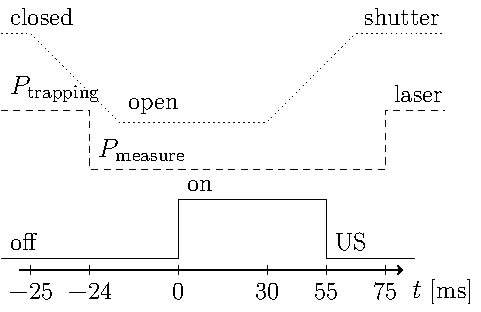
\includegraphics[]{Plots/cache/daq-sync.pdf}
  \caption{Schematic of controller timings for the shutter, the laser, and the 
      US. During the $P_{\text{measure}}$ state the particle is not trapped by 
  the OT. In the time interval $[\SI{0}{\ms}, \SI{30}{\ms}]$ (1) the shutter is 
  fully opened, (2) the US is switched on, and (3) the particle is free to 
  move. During this interval the measurement is performed.}\label{fig:TC-daq-sync}
\end{figure}

\subsection{Controller Timing and Data Acquisition}

The data acquisition (DAQ) board NI-USB 6356 (National Instruments, Austin, TX, 
USA), the laser power, the piezo excitation voltage, and the shutter 
transmittance are actuated in a defined sequence. We use an Arduino Board with 
two 12-Bit DAC units (MCP4725, Adafruit, New York, NY, USA) for controlling the 
timing and the DC voltage for the laser. The timings are depicted in 
\cref{fig:TC-daq-sync}. For $t<-\SI{24}{\ms}$ the laser is in its high power state 
and keeps the particle fixed in position against external forces. At 
$t=\SI{-25}{\ms}$ the shutter starts opening. The opening time is specified 
with less than \SI{15}{\ms} from 0\% transmittance to 90\%. At 
$t=\SI{-24}{\ms}$ the laser power changes to its low power state. Hence, the 
particle is free to move and starts its sedimentation. At $t=\SI{0}{\ms}$ the 
US is switched on. For \SI{30}{\ms} the shutter is fully opened, the particle 
is free to move, and the US is on. Then the shutter starts to close again. In 
these \SI{30}{\ms} we measure the time evolution of the particle. At 
$t=\SI{55}{\ms}$ the US is switched off and at $t=\SI{75}{\ms}$ the laser power 
is increased to its high power state. The time between two consecutive 
measurements is greater than \SI{2}{\s}, such that the fluid within the cavity 
is fully at rest again.

\subsection{Device, Particles, and Fluid}

Our device is a glass-silicon-glass device manufactured by Gesim GmbH 
(Radeberg, Germany). The material of the two glasses is B33 from Schott (Mainz, 
Germany). A sketch is shown in \cref{fig:TC-device} and its dimensions are listed 
in \cref{tab:TC-device-dimensions}. The top glass and the fluid cavity are limited 
in the $\ez$ direction because our microscope setup cannot focus deeper than 
\SI{250}{\um} \cite{Lamprecht2016,Lamprecht2017}. We define the origin of our 
coordinate system so that $z = 0$ is in the middle of the fluid cavity and $y = 
0$ is in the middle between the silicon cavity walls. We use as a reference 
point $x = 0$ such that it is approximately in the middle of the PZT length 
$l$. For all reported measurements we use the same position $x_{\text{ref}}$ as 
reference for $x=0$.

The fluid cavity is in the middle between the two silicon layers and the 
PZT is a PZ 26 element from Meggit A/S (Kvistgaard, 
Denmark). It is glued with Epo-Tek (Billerica, MA, USA) H20S two component 
epoxy onto the device. It is located at the edge of the device in $\ey$ 
direction and centered along the long side. The small height of 
the PZT is necessary to prevent physical contact with the microscope lens.

Our particles are silicon-dioxide (\SiO) particles from (microParticles GmbH, 
Berlin, Germany) with a diameter of $D_{2}=\SI{2.06}{\um}$. For the device 
characterization we also use particles from the same manufacturer with the same 
material properties, but with a diameter of $D_{4} = \SI{4.39}{\um}$. The 
particles are immersed in filtered (\SI{0.2}{\um}) and distilled water. To 
avoid particle-particle interactions during the experiment, we keep the 
particle concentration low.

We use the \Dtwo~particles because they are the smallest particles that work 
well in our OT. In addition, the critical radius where the ARF equals the drag 
force from AS can be found via \cite{Barnkob2012}
\begin{equation}
  \R_{\text{crit}} = \sqrt{\frac{3}{\Phi}}\,\delta
\end{equation}
where $\Phi$ is the acoustic contrast factor with thermoviscous correction 
\cite{Settnes2012}




\begin{subequations}
\begin{eqnarray}
  \Phi\left( \tkappa, \trho, \tdelta \right) &=& \frac{1}{3} f_{1}\left( 
  \tkappa \right) + \frac{1}{2}\,\text{Re}\left[ f_{2}\left( \trho, 
  \tdelta\right) \right],\\
  %%%%%%
  f_{1}\left( \tkappa \right) &=& 1 - \tkappa, \quad 
  \tkappa=\frac{\kappa_{\text{p}}}{\kappa_{\text{f}}},\\
  %%%%%%
  f_{2}\left( \trho, \tdelta \right) &=& \frac{2\left[ 1-\Gamma\left( \tdelta 
  \right) \right]\left( \trho-1 \right)}{2\,\trho + 1 - 3\,\Gamma\left( \tdelta 
  \right)}, \quad \trho=\frac{\rhop}{\rhof}\\
  %%%%%%
  \Gamma\left( \tdelta \right) &=& -\frac{3}{2}\left[ 1 + \iu \left( 1 + 
  \tdelta \right) \right]\tdelta, \, \tdelta = \frac{\delta}{R}, \, \delta = 
  \sqrt{\frac{\muef}{\rhof\,\pi f}}.
%
\end{eqnarray}
\end{subequations}
Here $\kappa_{\text{p}}$ is the particle and $\kappa_{\text{f}}$ the fluid 
compressibility, $\delta$ the viscous boundary layer thickness, and $\iu$ the 
imaginary unit. For our parameters (see \cref{tab:TC-parameters}) 
$\R_{\text{crit}} $ is equal to \SI{0.63}{\um} and \SI{0.65}{\um}, with and 
without ($\tdelta = 0$) thermoviscous correction, respectively.

With increasing particle size, two effects take place: 1) the ratio between ARF 
($\propto \R^{3}$) and AS ($\FAS\propto \R$) magnitude increases, because of 
their respective scaling, and 2) the measurement time decreases, because a 
greater ARF leads to more displacement, which in turn makes re-trapping more 
difficult.

% \begin{equation}
%   \delta = \sqrt{\frac{\muef}{\pi\,\rhof\,\fex}}
% \end{equation}

% \begin{equation}
%   \Phi = \frac{1}{3}\left[ \frac{5\,\tilde{\rho}-2}{2\,\tilde{\rho}+1} - 
%   \tilde{\kappa} \right]
% \end{equation}


